\section{Installation}
You have been provided a USB stick with all you will need for this tutorial. On
this drive is the following: 
\begin{itemize}
\item An ICE application for your operating system
\item A clone of the ICE git repository
\item All tutorial documentation and slides for today
\item Data files for the tutorial. 
\end{itemize}

\subsection{ICE Installation}
A number of files must first be copied from the USB stick to your local machine. Please
follow the steps below:
\begin{enumerate}
\item Choose a location that is easy to remember
and copy the correct \texttt{ice\-product*.zip} file for your computer's 
operation system (Linux, Mac OS X, or Windows).
\item Unzip this file to obtain the 
ICE application executable.
\item Copy the git repository \texttt{ice-repository.zip} file to your computer.
\item Unzip this file.
\end{enumerate}

\subsection{Starting ICE for the first time}
To start ICE, double-click on the application executable to open up ICE. When the workspace chooser
dialog opens, select the default workspace by clicking on the \texttt{OK}
button.
You can enter your own directory for the workspace location, but please make sure that it is writable and readable by you, and you remember where it is.
\begin{center} 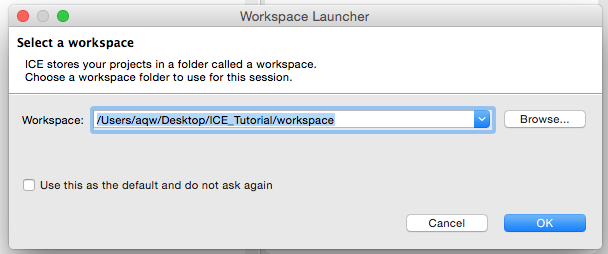
\includegraphics[width=\textwidth]{figures/workspace}
\end{center}
When ICE opens you should see an empty \texttt{Plug-in Development} perspective
similar to the image below.
\begin{center} 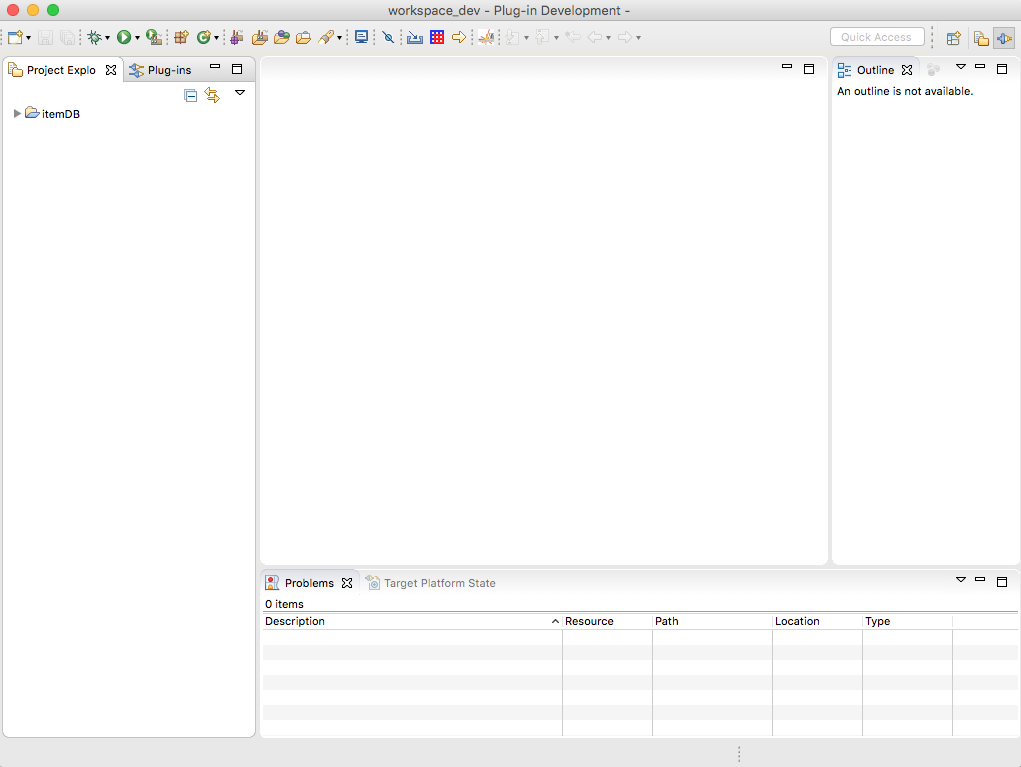
\includegraphics[width=\textwidth]{figures/expectedICE}
\end{center} 

\subsection{Setting up ICE}
In order to create a dashboard for your application, you will need to configure ICE to
be able to develop ICE. This \textit{Software Development Kit (SDK) version} of
ICE will contain all the components necessary to generate a new instance of ICE that will become your application's dashboard. 
The first step in doing this is to load the ICE bundles into
your workspace. We have provided a developer menu to assist in this process:

\begin{enumerate}
\item Select \texttt{Developer $\rightarrow$ ICE $\rightarrow$
Import Local Repository}
\item Using the directory dialog, navigate to the git repository you copied
from the USB drive.
\item Select \texttt{Open}
\item In the \texttt{Search results} list, select the checkbox next to the
repository
\item Select \texttt{Finish}
\end{enumerate}

This should import all the ICE bundles and you should have something
like the image below.
\begin{center} 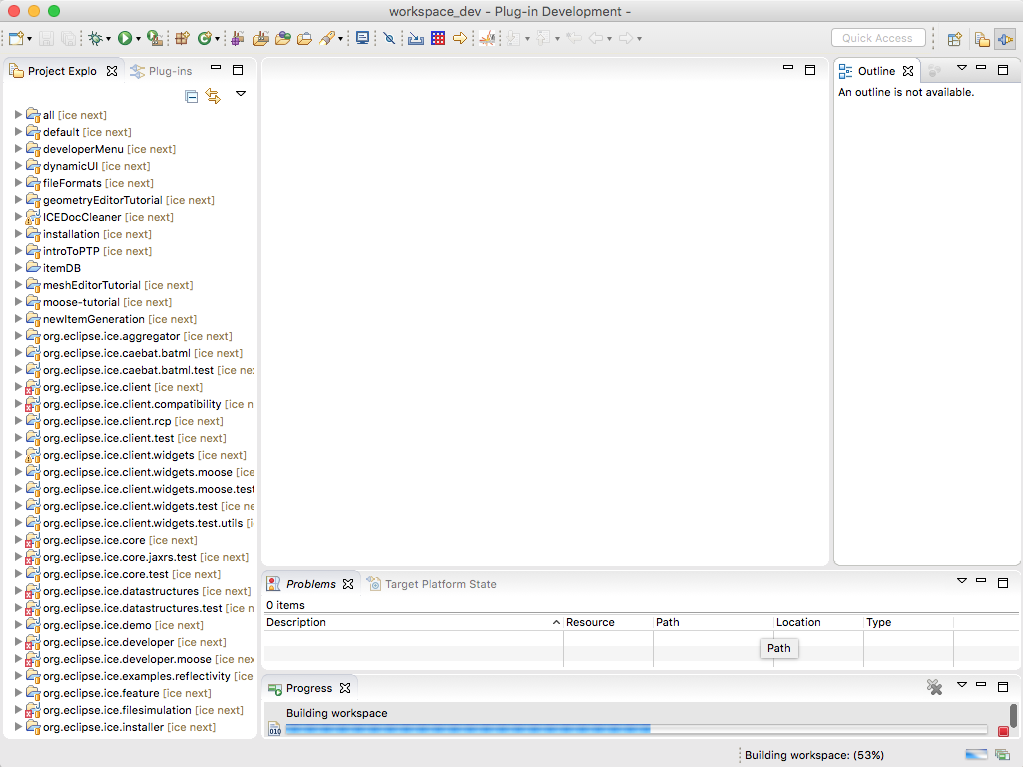
\includegraphics[width=\textwidth]{figures/cloned} \end{center}

At this point, you are ready to begin developing a dashboard for your
application!
